\documentclass[11pt,a4paper]{article}

% --- Packages ---
\usepackage[margin=2.5cm]{geometry}
\usepackage{amsmath,amssymb}
\usepackage{booktabs}
\usepackage{graphicx}
\usepackage{hyperref}
\usepackage{xcolor}
\usepackage{fancyhdr}
\usepackage{microtype}
\usepackage{caption}
\usepackage{subcaption}
\usepackage{multirow}
\usepackage{array}
\usepackage{enumitem}
\usepackage{cite}
\usepackage{pgfplots}
\usepackage{pgfplotstable}
\pgfplotsset{compat=1.18}
\usepackage{tikz}

% --- WIP Footer (fancyhdr) ---
\pagestyle{fancy}
\fancyhf{}
\fancyfoot[L]{\small\textit{This research is ongoing}}
\fancyfoot[C]{\thepage}
\fancyfoot[R]{\small\textit{AtomGradient}}
\renewcommand{\headrulewidth}{0pt}
\fancypagestyle{plain}{%
  \fancyhf{}
  \fancyfoot[L]{\small\textit{This research is ongoing}}
  \fancyfoot[C]{\thepage}
  \fancyfoot[R]{\small\textit{AtomGradient}}
  \renewcommand{\headrulewidth}{0pt}
}

% --- Hyperref setup ---
\hypersetup{
  colorlinks=true,
  linkcolor=blue!60!black,
  citecolor=blue!60!black,
  urlcolor=blue!60!black,
  pdftitle={Efficient On-Device LLM Inference on Apple Silicon: From Quantization to Speculative Decoding},
  pdfauthor={AtomGradient}
}

% --- Custom commands ---
\newcommand{\tps}{\,tok/s}
\newcommand{\SD}{speculative decoding}

% ============================================================
\begin{document}
% ============================================================

\title{\textbf{Efficient On-Device LLM Inference on Apple Silicon:\\
From Quantization to Speculative Decoding}}

\author{\textit{AtomGradient}}
\date{March 2026}

\maketitle
\thispagestyle{plain}

% ============================================================
\begin{abstract}
% ============================================================
We present a systematic empirical study of large language model (LLM) inference
efficiency on Apple Silicon unified-memory devices, covering post-training
quantization (PTQ), quantization-aware training (QAT), and speculative decoding
(SD).
Using Qwen3.5-4B as our primary subject under llama.cpp GGUF quantization,
we find that Q8\_0 achieves near-lossless compression (0.18\% perplexity
degradation, 1.47$\times$ token-generation speedup), Q6\_K is the Pareto-optimal
production choice (0.54\% degradation, 1.68$\times$ speedup, 59\% size
reduction), and Q4\_K\_M suits memory-constrained deployments (4.07\%
degradation, 68\% size reduction).
Sub-4-bit quantization degrades quality catastrophically (267\% PPL increase for
Q2\_K) with marginal throughput gains.
For \SD, we discover that on Apple Silicon the critical predictor is the
draft-to-target speed ratio rather than acceptance rate: a 0.8B draft model
(140 tok/s) paired with a 9B target (42.4 tok/s) yields a 3.3$\times$ speed ratio
and achieves 25.7\% throughput improvement at only 2--4\% acceptance rates,
owing to Metal GPU batch-verification efficiency.
Self-speculative decoding (same model at lower quantization) is ineffective when
the speed ratio falls below 2.5$\times$.
Mixture-of-Experts models, already memory-efficient due to sparse activation
(\textasciitilde3B of 35B parameters active per token), receive no benefit from
\SD.
We further conduct cross-device \SD\ experiments using GGML\_RPC over a Gigabit
LAN, routing draft model compute to remote M1 Max and M2 Pro machines.
Corrected measurements reveal $\sim$79--83\% throughput reduction, driven by
per-op RPC protocol overhead ($\sim$51--57~ms per draft token) rather than
network bandwidth; the current GGML\_RPC implementation is not viable for
production cross-device inference.
\end{abstract}

\tableofcontents
\newpage

% ============================================================
\section{Introduction}
% ============================================================

The deployment of large language models on consumer and edge devices has gained
significant momentum as chip vendors integrate high-bandwidth unified memory
with powerful neural accelerators.
Apple Silicon---in particular, the M-series chips---combines CPU, GPU, and Neural
Engine on a single die with a unified memory pool, enabling in-context model
sizes that would require a dedicated GPU on conventional hardware.
Understanding how to maximize inference efficiency on this architecture is both
practically relevant and scientifically interesting, as several well-known
optimization techniques developed for discrete GPU pipelines behave differently
on unified memory.

This paper makes five concrete contributions:

\begin{enumerate}[leftmargin=*, label=\textbf{\arabic*.}]
  \item \textbf{Quantization ladder benchmark.}
    We benchmark Qwen3.5-4B across seven GGUF quantization levels (F16 through
    Q2\_K) on an M2 Ultra, measuring token-generation throughput and WikiText-2
    perplexity at each level.
    We identify a quality ``elbow'' at Q4\_K\_M and a performance ``elbow'' near
    Q6\_K.

  \item \textbf{QAT vs.\ PTQ comparison.}
    We compare Gemma-3-4B quantization-aware training variants (3/4/6/8-bit)
    against Qwen3.5-4B post-training quantization under the MLX framework,
    showing that QAT exhibits smoother throughput gradients with minimal variance.

  \item \textbf{Speed ratio as the key predictor for speculative decoding.}
    We show that on Apple Silicon, speculative decoding benefit is governed by
    the draft-to-target speed ratio (not acceptance rate): any ratio $\geq 2.5\times$
    yields positive throughput gain even at 2--4\% acceptance rates, due to
    fixed-cost batch verification on Metal GPU.

  \item \textbf{Self-speculative decoding and MoE incompatibility.}
    We demonstrate that (a) same-model-different-quantization self-speculation is
    ineffective on unified memory due to insufficient speed ratios, and
    (b) MoE models (Qwen3.5-35B-A3B) already operate at throughput comparable
    to small dense models and thus receive no benefit from \SD.

  \item \textbf{Cross-device speculative decoding via GGML\_RPC.}
    We evaluate routing draft model compute to remote Apple Silicon machines
    (M1 Max, M2 Pro) via GGML\_RPC over a Gigabit LAN, including a careful
    investigation of measurement validity (silent local fallback in BLAS builds).
    Corrected measurements show $\sim$79--83\% throughput reduction, dominated by
    per-op RPC protocol overhead; current GGML\_RPC is not viable for production
    cross-device SD and a purpose-built streaming protocol is needed.
\end{enumerate}

% ============================================================
\section{Background}
% ============================================================

\subsection{Apple Silicon Unified Memory Architecture}

Unlike discrete GPU systems where model weights must be transferred over PCIe
($\sim$64~GB/s), Apple Silicon's unified memory allows the GPU to access model
weights at full memory bus bandwidth.
Table~\ref{tab:hardware} summarizes the key hardware parameters of the machines
used in this study.

\begin{table}[h]
\centering
\caption{Hardware specifications of test machines.}
\label{tab:hardware}
\begin{tabular}{llllr}
\toprule
\textbf{Machine} & \textbf{Chip} & \textbf{Memory} & \textbf{BW} & \textbf{GPU Cores} \\
\midrule
M2 Ultra & Apple M2 Ultra & 192 GB & 800 GB/s & 76 \\
M1 Max   & Apple M1 Max   &  32 GB & 400 GB/s & 32 \\
M2 Pro   & Apple M2 Pro   &  32 GB & 200 GB/s & 19 \\
\bottomrule
\end{tabular}
\end{table}

Token generation (TG) is a memory-bandwidth-bound operation: each forward pass
loads nearly all model weights from memory to compute a single token.
With 76 GPU cores and 800 GB/s bandwidth, the M2 Ultra is particularly suited
for memory-bound inference.
Prompt processing (PP), by contrast, processes many tokens in parallel and is
compute-bound.

\subsection{Post-Training Quantization (PTQ)}

PTQ reduces model precision after training, trading representation fidelity for
reduced memory footprint and higher memory bandwidth utilization.
GGUF~\cite{gguf} (used in llama.cpp) supports a range of k-quant formats:
Q2\_K, Q3\_K\_M, Q4\_K\_M, Q5\_K\_M, Q6\_K, Q8\_0, and F16.
Higher-bit formats preserve more information but require more memory bandwidth
per token.

\subsection{Quantization-Aware Training (QAT)}

QAT incorporates quantization into the training loop, allowing the model to
adapt its weights to the precision constraints.
Gemma-3-4B~\cite{gemma3} provides official QAT checkpoints at 3, 4, 6, and 8
bits, evaluated here via the MLX framework~\cite{mlx}.

\subsection{Speculative Decoding}

Speculative decoding~\cite{leviathan2023fast,chen2023accelerating} uses a small
``draft'' model to propose $k$ candidate tokens, which the large ``target'' model
verifies in a single forward pass.
If the target accepts the draft's tokens, effective throughput increases.
The theoretical speedup depends on the acceptance rate $\alpha$ and the
draft-to-target cost ratio.
On discrete GPUs, verification is cheap because the GPU processes batches
efficiently; on unified memory, we hypothesize similar behavior due to Metal GPU
batch-processing.

% ============================================================
\section{Experimental Setup}
% ============================================================

\subsection{Models and Tools}

\textbf{Primary model:} Qwen3.5-4B~\cite{qwen35} in GGUF format, quantized from
an F16 base generated via \texttt{convert\_hf\_to\_gguf.py} from the
HuggingFace safetensors checkpoint.

\textbf{Additional models:}
\begin{itemize}
  \item Qwen3.5-0.8B, -2B, -9B (GGUF Q8\_0) --- benchmarked on all three machines
  \item Qwen3.5-35B-A3B (GGUF Q4\_K\_XL and Q8\_0, MoE) --- M2 Ultra only (fits in 192~GB)
  \item Gemma-3-4B QAT at 3/4/6/8-bit (MLX)
  \item Qwen3-8B at 3/4/6-bit (MLX)
\end{itemize}

\textbf{Inference engines:}
\begin{itemize}
  \item \texttt{llama-bench} --- throughput benchmarking (N\_PROMPT=512, N\_GEN=128, 4 runs)
  \item \texttt{llama-perplexity} --- WikiText-2 perplexity (--chunks 10, ctx=512)
  \item \texttt{llama-speculative} --- speculative decoding (N\_PREDICT=200, T=0)
  \item \texttt{mlx\_lm.generate} --- MLX framework inference (N\_GEN=128, 3 runs)
  \item \texttt{rpc-server} (GGML\_RPC=ON) --- remote draft backend for cross-device SD
\end{itemize}

\subsection{Quantization Pipeline}

Starting from the Qwen3.5-4B HuggingFace checkpoint (bf16 safetensors), we:
{\sloppy
\begin{enumerate}
  \item Converted to GGUF F16 via \texttt{convert\_hf\_to\_gguf.py}
  \item Quantized to Q8\_0, Q6\_K, Q5\_K\_M, Q4\_K\_M, Q3\_K\_M,
        and Q2\_K via \texttt{llama-quantize}
\end{enumerate}
}

Note: The Qwen3.5-9B model is available only as a Unsloth Dynamic (UD) Q8\_K\_XL
variant, whose \texttt{q8\_0} tensor format cannot be requantized by
\texttt{llama-quantize}; hence the 4B series was used for the quantization
ladder experiment.

% ============================================================
\section{Experiments}
% ============================================================

\subsection{Quantization Throughput Benchmark}

Table~\ref{tab:quant_tg} reports token-generation and prompt-processing
throughput for Qwen3.5-4B across all quantization levels on the M2 Ultra.

\begin{table}[h]
\centering
\caption{Qwen3.5-4B throughput across quantization levels (M2 Ultra 192 GB).
TG = token generation (memory-bandwidth-bound);
PP = prompt processing (compute-bound).}
\label{tab:quant_tg}
\begin{tabular}{lrrrr}
\toprule
\textbf{Quant} & \textbf{TG (tok/s)} & \textbf{PP (tok/s)} & \textbf{Size (GB)} & \textbf{TG/$_{\text{F16}}$} \\
\midrule
F16     & 36.8  & 1931.6 & 8.42 & 1.00$\times$ \\
Q8\_0   & 54.0  & 1373.6 & 4.48 & 1.47$\times$ \\
Q6\_K   & 62.0  & 1358.9 & 3.46 & 1.68$\times$ \\
Q5\_K\_M & 56.6  & 1276.1 & 3.11 & 1.54$\times$ \\
Q4\_K\_M & 58.5  & 1337.6 & 2.71 & 1.59$\times$ \\
Q3\_K\_M & 68.8  & 1611.9 & 2.26 & 1.87$\times$ \\
Q2\_K   & 72.8  & 1700.9 & 1.80 & 1.98$\times$ \\
\bottomrule
\end{tabular}
\end{table}

\textbf{TG observation.}
Token-generation speed increases monotonically as quantization is reduced,
confirming the memory-bandwidth-bound hypothesis: Q2\_K loads $\sim$4.7$\times$
fewer bytes per weight than F16, yielding a 1.98$\times$ speedup.
The non-linear relationship (e.g., Q8\_0 is faster than Q6\_K might suggest,
yet Q5\_K\_M is slower than Q4\_K\_M) reflects varying dequantization kernel
efficiency for different k-quant formats on Metal GPU.

\textbf{PP observation.}
Prompt processing exhibits a U-shaped curve: F16 achieves the highest PP
(1931 tok/s) because there is no dequantization overhead; mid-precision formats
(Q4--Q6) are slowest; Q2/Q3 partially recovers speed, likely because the
corresponding Metal GPU kernels benefit from more compact SIMD packing at very
low bit-widths---the activation matrices remain the same size regardless of
weight precision.

Figure~\ref{fig:quant_tg_ppl} visualizes the trade-off between throughput and
perplexity across quantization levels.

\begin{figure}[h]
\centering
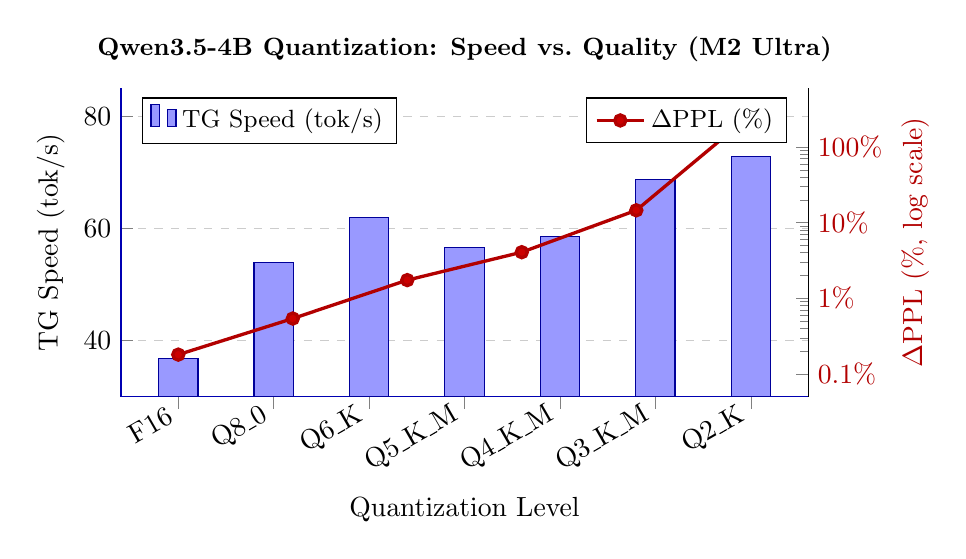
\begin{tikzpicture}
\begin{axis}[
  width=0.85\linewidth, height=5.5cm,
  xlabel={Quantization Level},
  ylabel={TG Speed (tok/s)},
  xtick={1,2,3,4,5,6,7},
  xticklabels={F16,Q8\_0,Q6\_K,Q5\_K\_M,Q4\_K\_M,Q3\_K\_M,Q2\_K},
  xticklabel style={rotate=30, anchor=east},
  ymin=30, ymax=85,
  axis y line*=left,
  axis x line*=bottom,
  bar width=0.5cm,
  ybar,
  fill=blue!40!white,
  draw=blue!70!black,
  ymajorgrids=true,
  grid style={dashed, gray!40},
  legend pos=north west,
  legend style={font=\small},
  title={Qwen3.5-4B Quantization: Speed vs.\ Quality (M2 Ultra)},
  title style={font=\small\bfseries},
]
\addplot[ybar, fill=blue!40, draw=blue!60!black]
  coordinates {(1,36.8) (2,54.0) (3,62.0) (4,56.6) (5,58.5) (6,68.8) (7,72.8)};
\addlegendentry{TG Speed (tok/s)}
\end{axis}
\begin{axis}[
  width=0.85\linewidth, height=5.5cm,
  xtick={1,2,3,4,5,6,7},
  xticklabels={F16,Q8\_0,Q6\_K,Q5\_K\_M,Q4\_K\_M,Q3\_K\_M,Q2\_K},
  xticklabel style={rotate=30, anchor=east},
  ylabel={$\Delta$PPL (\%, log scale)},
  ylabel style={color=red!70!black},
  ymode=log,
  ymin=0.05, ymax=600,
  ytick={0.1,1,10,100},
  yticklabels={0.1\%,1\%,10\%,100\%},
  yticklabel style={color=red!70!black},
  axis y line*=right,
  axis x line=none,
  legend pos=north east,
  legend style={font=\small},
]
% F16 baseline (0%) omitted as log(0) is undefined; Q8_0 onward plotted
\addplot[red!70!black, very thick, mark=*, mark options={fill=red!80!black}]
  coordinates {(2,0.18) (3,0.54) (4,1.74) (5,4.07) (6,14.57) (7,267)};
\addlegendentry{$\Delta$PPL (\%)}
\end{axis}
\end{tikzpicture}
\caption{Token-generation throughput (bars, left axis) vs.\ perplexity degradation
$\Delta$PPL\% from F16 baseline (line, right \emph{log} axis) for Qwen3.5-4B.
F16 is omitted from the PPL line (baseline = 0\%, undefined on log scale).
The log scale reveals the sharp quality cliff at Q3/Q2.}
\label{fig:quant_tg_ppl}
\end{figure}

\subsection{Quality vs.\ Quantization: Perplexity Evaluation}

Table~\ref{tab:ppl} reports WikiText-2 perplexity and a composite efficiency
score (TG speedup / \%PPL degradation) for each quantization level.

\begin{table}[h]
\centering
\caption{Perplexity (WikiText-2 test, chunks=10, ctx=512) for Qwen3.5-4B.
$\Delta$PPL\% = relative degradation from F16 baseline (PPL\,=\,11.055).
TG speedup from Table~\ref{tab:quant_tg}.}
\label{tab:ppl}
\begin{tabular}{lrrrr}
\toprule
\textbf{Quant} & \textbf{PPL} & \textbf{$\Delta$PPL} & \textbf{$\Delta$PPL\%} & \textbf{TG Speedup} \\
\midrule
F16      & 11.055 $\pm$ 0.604 & ---    & ---     & 1.00$\times$ \\
Q8\_0    & 11.075 $\pm$ 0.605 & +0.020 & 0.18\%  & 1.47$\times$ \\
Q6\_K    & 11.115 $\pm$ 0.607 & +0.060 & 0.54\%  & 1.68$\times$ \\
Q5\_K\_M & 11.248 $\pm$ 0.619 & +0.193 & 1.74\%  & 1.54$\times$ \\
Q4\_K\_M & 11.504 $\pm$ 0.634 & +0.449 & 4.07\%  & 1.59$\times$ \\
Q3\_K\_M & 12.668 $\pm$ 0.713 & +1.613 & 14.57\% & 1.87$\times$ \\
Q2\_K    & 40.602 $\pm$ 2.632 & +29.55 & 267\%   & 1.98$\times$ \\
\bottomrule
\end{tabular}
\end{table}

\textbf{Key observations.}
Q8\_0 is essentially lossless (0.18\% PPL degradation) and achieves the highest
efficiency score (8.2).
Q6\_K is the Pareto-optimal production deployment choice, offering 0.54\% quality
loss with 1.68$\times$ speedup and 59\% size reduction.
Q5\_K\_M is dominated by Q6\_K on both dimensions and should generally be avoided.
Q3\_K\_M shows a quality cliff ($\Delta$PPL jumps from 4.07\% to 14.57\%) with
only 18\% additional throughput over Q4\_K\_M, making it rarely worthwhile.
Q2\_K is practically unusable: PPL of 40.6 indicates degenerate outputs.

\subsection{QAT vs.\ PTQ: MLX Framework Comparison}

Table~\ref{tab:qat} compares Gemma-3-4B QAT (official checkpoints) against
Qwen3.5-4B PTQ under the MLX framework on the M2 Ultra.
Note that Gemma-3 and Qwen3.5 are different model families with different
architectures and training data; this comparison characterises the throughput
behaviour of the QAT vs.\ PTQ technique rather than the relative quality of
the two models.

\begin{table}[h]
\centering
\caption{Gemma-3-4B QAT throughput on M2 Ultra 192 GB (MLX, N\_GEN=128, 3 runs).
QAT = quantization-aware training.}
\label{tab:qat}
\begin{tabular}{lrrl}
\toprule
\textbf{Model} & \textbf{TG (tok/s)} & \textbf{Size (MB)} & \textbf{Notes} \\
\midrule
Gemma-3-4B QAT 3bit & 137.3 $\pm$ 0.3 & 2871 & --- \\
Gemma-3-4B QAT 4bit & 119.0 $\pm$ 0.1 & 3049 & --- \\
Gemma-3-4B QAT 6bit & 107.2 $\pm$ 0.2 & 4578 & --- \\
Gemma-3-4B QAT 8bit &  96.4 $\pm$ 0.2 & 5716 & --- \\
\midrule
Qwen3.5-4B Q4\_K\_M & 58.5  & 2713 & PTQ, llama.cpp \\
Qwen3.5-4B (bf16)   & 59.3  & 9343 & MLX, full precision \\
\bottomrule
\end{tabular}
\end{table}

QAT models exhibit remarkably smooth throughput gradients (3-bit to 8-bit spans
137 to 96 tok/s, a 1.42$\times$ range) with near-zero variance ($\sigma < 0.3$
tok/s).
This stability is attributed to the model having adapted to quantization noise
during training, producing more numerically well-conditioned weight distributions.
By contrast, Qwen3-8B PTQ 3/4-bit show $\sigma \approx 19$ tok/s, likely due to
MLX compute-graph caching artifacts with these specific model sizes.

\subsection{Multi-Size Scaling on Apple Silicon}

Table~\ref{tab:multisize} shows how throughput scales across model sizes on the
M2 Ultra, along with a hardware comparison for the 9B model.

\begin{table}[h]
\centering
\caption{Multi-size Qwen3.5 throughput on M2 Ultra 192 GB (GGUF, llama-bench).
The 35B-A3B MoE model activates only $\sim$3B parameters per token.}
\label{tab:multisize}
\begin{tabular}{lrrr}
\toprule
\textbf{Model} & \textbf{TG (tok/s)} & \textbf{PP (tok/s)} & \textbf{Size (GB)} \\
\midrule
Qwen3.5-0.8B Q8\_0             & 140.2 &  7410.7 & 1.19 \\
Qwen3.5-2B Q8\_0               & 110.6 &  4469.2 & 2.83 \\
Qwen3.5-4B Q4\_K\_M            &  58.5 &  1337.6 & 2.71 \\
Qwen3.5-9B Q8\_0               &  42.4 &  1163.9 & 12.97 \\
Qwen3.5-35B-A3B Q8\_0 (MoE)   & \textbf{50.0} & 1530.5 & 36.0 \\
\bottomrule
\end{tabular}
\end{table}

The MoE model (Qwen3.5-35B-A3B) achieves 50.0 tok/s at Q8\_0 despite its 36 GB
size, because only $\sim$3B of its 35B parameters are activated per token.
This makes it bandwidth-comparable to a dense 3B model, explaining its
anomalously high throughput.

Table~\ref{tab:hw_compare} extends the hardware comparison to three machines on
the same Qwen3.5-9B Q8\_0 model.

\begin{table}[h]
\centering
\caption{Three-machine hardware comparison on Qwen3.5-9B Q8\_0.
BW util.\ = TG $\times$ 12.07\,GB / mem.\ BW, where 12.07\,GB is the
actual weight payload (file size is 12.97\,GB including GGUF metadata).}
\label{tab:hw_compare}
\begin{tabular}{lrrrr}
\toprule
\textbf{Machine} & \textbf{Mem.\ BW} & \textbf{TG (tok/s)} & \textbf{PP (tok/s)} & \textbf{BW util.} \\
\midrule
M2 Ultra (192 GB) & 800 GB/s & 42.4 & 1163.9 & 64\% \\
M1 Max (32 GB)    & 400 GB/s & 21.8 &  483.7 & 66\% \\
M2 Pro (32 GB)    & 200 GB/s & 12.7 &  321.3 & 77\% \\
\bottomrule
\end{tabular}
\end{table}

TG throughput scales approximately linearly with memory bandwidth (M2 Ultra:
M1 Max:\ M2 Pro $\approx$ 3.3:1.7:1, vs.\ BW ratio 4:2:1), confirming
the memory-bandwidth-bound nature of token generation.
The M2 Pro shows slightly higher BW utilization (77\%) relative to its lower core
count, likely due to a more favourable weight-to-bandwidth ratio at 200 GB/s.
The 35B-A3B MoE model requires 36 GB of unified memory and was only benchmarked
on the M2 Ultra.

Figure~\ref{fig:hw_compare} shows TG speeds across all three machines and model
sizes.

\begin{figure}[h]
\centering
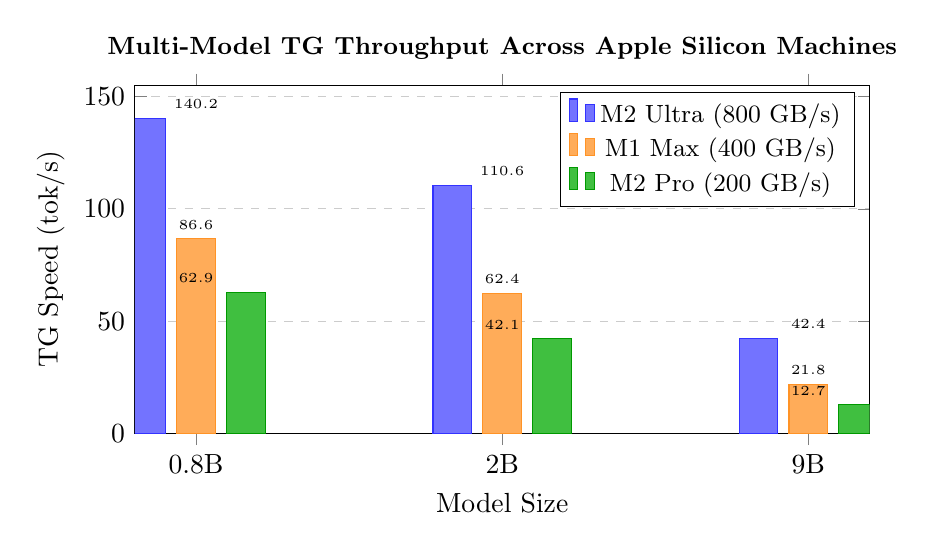
\begin{tikzpicture}
\begin{axis}[
  width=0.9\linewidth, height=6cm,
  xlabel={Model Size},
  ylabel={TG Speed (tok/s)},
  symbolic x coords={0.8B,2B,9B},
  xtick=data,
  ymin=0, ymax=155,
  ybar=4pt,
  bar width=14pt,
  ymajorgrids=true,
  grid style={dashed, gray!40},
  legend style={at={(0.98,0.98)}, anchor=north east, font=\small},
  title={Multi-Model TG Throughput Across Apple Silicon Machines},
  title style={font=\small\bfseries},
  nodes near coords,
  nodes near coords style={font=\tiny, rotate=90, anchor=west},
  every node near coord/.style={font=\tiny},
]
\addplot[fill=blue!55, draw=blue!80]
  coordinates {(0.8B,140.2) (2B,110.6) (9B,42.4)};
\addlegendentry{M2 Ultra (800 GB/s)}
\addplot[fill=orange!65, draw=orange!85]
  coordinates {(0.8B,86.6) (2B,62.4) (9B,21.8)};
\addlegendentry{M1 Max (400 GB/s)}
\addplot[fill=green!50!gray, draw=green!60!black]
  coordinates {(0.8B,62.9) (2B,42.1) (9B,12.7)};
\addlegendentry{M2 Pro (200 GB/s)}
\end{axis}
\end{tikzpicture}
\caption{Token-generation throughput (tok/s) for Qwen3.5 Q8\_0 models across
three Apple Silicon machines. Throughput scales approximately with memory bandwidth.}
\label{fig:hw_compare}
\end{figure}

\subsection{Speculative Decoding Experiments}

\subsubsection{Effect of Draft Model Size (9B Target)}

Table~\ref{tab:sd_9b} reports speculative decoding results with the 9B Q8\_0
target and two draft models.

\begin{table}[h]
\centering
\caption{Speculative decoding with Qwen3.5-9B Q8\_0 target (baseline: 42.4 tok/s).
Speed ratio = draft TPS / target TPS. Results averaged over code, text, and math prompts.}
\label{tab:sd_9b}
\begin{tabular}{llrrrr}
\toprule
\textbf{Draft} & $k$ & \textbf{Speed Ratio} & \textbf{Avg Accept\%} & \textbf{Avg TPS} & \textbf{$\Delta$Baseline} \\
\midrule
0.8B Q8\_0 & 4 & 3.31$\times$ & 3.3\% & 53.3 & \textbf{+25.7\%} \\
0.8B Q8\_0 & 8 & 3.31$\times$ & 1.3\% & 52.7 & +24.3\% \\
2B Q8\_0   & 4 & 2.61$\times$ & 3.4\% & 48.5 & +14.3\% \\
2B Q8\_0   & 8 & 2.61$\times$ & 1.4\% & 47.8 & +12.7\% \\
\bottomrule
\end{tabular}
\end{table}

\textbf{Speed ratio dominates acceptance rate.}
Despite the 0.8B draft having similar (even slightly lower) acceptance rates
compared to the 2B draft, it achieves 11\% more speedup.
The 0.8B model runs at 140 tok/s vs.\ the 9B target at 42.4 tok/s
(ratio = 3.31$\times$), while the 2B model achieves only 2.61$\times$.
This confirms that on Apple Silicon, the draft model's speed relative to the
target is the primary determinant of SD benefit.

\textbf{Even at 2--4\% acceptance rates, SD is beneficial.}
The Metal GPU batch-verification mechanism processes $k+1$ tokens in
approximately the same wall-clock time as a single token verification,
making the verification cost nearly independent of $k$.
Therefore, even if only 1--2 tokens out of $k$ are accepted, the effective
throughput increases.

Figure~\ref{fig:sd_speedratio} illustrates the relationship between draft-target
speed ratio and measured throughput speedup across all SD experiments.

\begin{figure}[h]
\centering
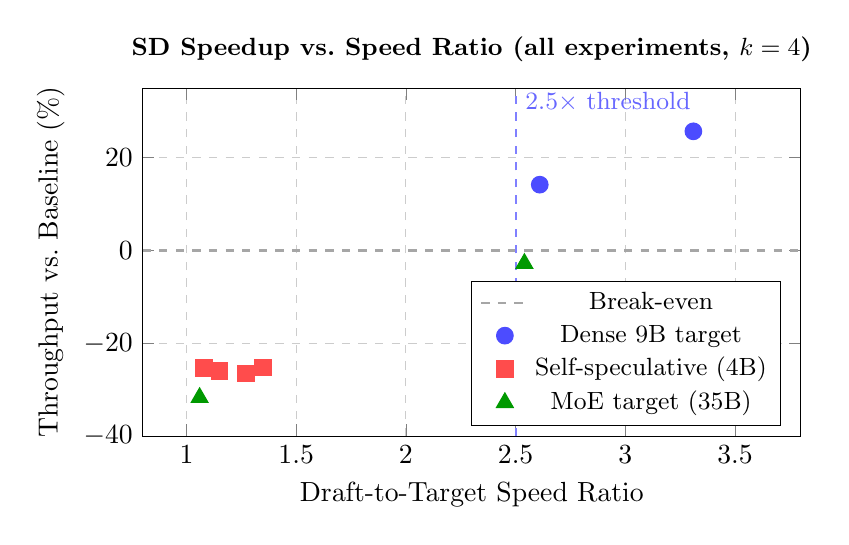
\begin{tikzpicture}
\begin{axis}[
  width=0.82\linewidth, height=6cm,
  xlabel={Draft-to-Target Speed Ratio},
  ylabel={Throughput vs.\ Baseline (\%)},
  xmin=0.8, xmax=3.8,
  ymin=-40, ymax=35,
  ymajorgrids=true, xmajorgrids=true,
  grid style={dashed, gray!40},
  legend pos=south east,
  legend style={font=\small},
  title={SD Speedup vs.\ Speed Ratio (all experiments, $k=4$)},
  title style={font=\small\bfseries},
]
% Horizontal break-even line
\addplot[dashed, gray!70, thick] coordinates {(0.8,0) (3.8,0)};
\addlegendentry{Break-even}

% Dense target experiments (9B target)
\addplot[blue!70, mark=*, mark size=3pt, only marks]
  coordinates {(3.31,25.7) (2.61,14.2)};
\addlegendentry{Dense 9B target}

% Self-speculative (4B target)
\addplot[red!70, mark=square*, mark size=3pt, only marks]
  coordinates {(1.35,-25.2) (1.27,-26.5) (1.08,-25.3) (1.15,-25.9)};
\addlegendentry{Self-speculative (4B)}

% MoE target
\addplot[green!60!black, mark=triangle*, mark size=3.5pt, only marks]
  coordinates {(2.54,-2.8) (1.06,-31.7)};
\addlegendentry{MoE target (35B)}

% Threshold line at 2.5x
\addplot[dashed, blue!50, thick] coordinates {(2.5,-40) (2.5,35)};
\node[blue!60, font=\small] at (axis cs:2.5,32) [anchor=west] {$2.5\times$ threshold};

\end{axis}
\end{tikzpicture}
\caption{Throughput change vs.\ baseline as a function of draft-to-target speed
ratio, for all $k=4$ speculative decoding experiments.
A speed ratio of $\geq 2.5\times$ reliably produces positive speedup regardless
of target model type; below this threshold, SD degrades performance.}
\label{fig:sd_speedratio}
\end{figure}

Table~\ref{tab:sd_9b_prompt} breaks down the 0.8B $\rightarrow$ 9B results by
prompt type.

\begin{table}[h]
\centering
\caption{SD results by prompt type: 0.8B Q8\_0 draft $\rightarrow$ 9B Q8\_0 target, $k=4$.}
\label{tab:sd_9b_prompt}
\begin{tabular}{lrrr}
\toprule
\textbf{Prompt Type} & \textbf{Accept\%} & \textbf{TPS} & \textbf{vs.\ Baseline} \\
\midrule
Code & 4.4\% & 55.1 & +30.0\% \\
Math & 3.2\% & 53.6 & +26.4\% \\
Text & 2.3\% & 51.2 & +20.8\% \\
\bottomrule
\end{tabular}
\end{table}

Code prompts yield the highest acceptance rates (4.4\%), reflecting the
deterministic, pattern-heavy nature of code completions that smaller models
predict more reliably than free-form text.

\subsubsection{Self-Speculative Decoding (Same Model, Lower Quantization)}

Table~\ref{tab:sd_self} shows results for self-speculative decoding using the
4B Q8\_0 as target and various lower-precision 4B variants as draft.

\begin{table}[h]
\centering
\caption{Self-speculative decoding: Qwen3.5-4B Q8\_0 target (baseline: 54.0 tok/s), $k=4$.
All draft models are the same architecture at lower precision.}
\label{tab:sd_self}
\begin{tabular}{lrrrr}
\toprule
\textbf{Draft Quant} & \textbf{Draft TPS} & \textbf{Speed Ratio} & \textbf{Avg TPS} & \textbf{$\Delta$Baseline} \\
\midrule
Q6\_K & 62.0 & 1.15$\times$ & 40.1 & $-$25.7\% \\
Q4\_K\_M & 58.5 & 1.08$\times$ & 40.4 & $-$25.2\% \\
Q3\_K\_M & 68.8 & 1.27$\times$ & 39.7 & $-$26.5\% \\
Q2\_K   & 72.8 & 1.35$\times$ & 40.4 & $-$25.2\% \\
\bottomrule
\end{tabular}
\end{table}

All self-speculative configurations reduce throughput by $\sim$25\%, regardless
of the draft quantization level.
The root cause is that even the fastest variant (Q2\_K at 72.8 tok/s) achieves
only a 1.35$\times$ speed ratio over the Q8\_0 target (54.0 tok/s).
On Apple Silicon unified memory, the verification overhead---loading both draft
and target model weights---requires a speed ratio of at least 2.5$\times$ to
yield net benefit.
This contrasts with discrete GPU architectures, where the verification step is
more efficiently parallelized across thousands of CUDA cores.

\subsubsection{MoE Target Model (35B Q4\_K\_XL)}

Table~\ref{tab:sd_moe} reports SD results with the 35B MoE target.

\begin{table}[h]
\centering
\caption{Speculative decoding with Qwen3.5-35B-A3B Q4\_K\_XL MoE target (baseline: 55.2 tok/s), $k=4$.}
\label{tab:sd_moe}
\begin{tabular}{lrrrr}
\toprule
\textbf{Draft} & \textbf{Speed Ratio} & \textbf{Avg Accept\%} & \textbf{Avg TPS} & \textbf{$\Delta$Baseline} \\
\midrule
0.8B Q8\_0 & 2.54$\times$ & 2.9\% & 53.7 & $-$2.8\% \\
4B Q4\_K\_M & 1.06$\times$ & 2.7\% & 37.7 & $-$31.7\% \\
\bottomrule
\end{tabular}
\end{table}

The MoE model represents a boundary case: with a 2.54$\times$ speed ratio, the
0.8B draft yields near-zero change ($-$2.8\%), while all smaller ratios cause
significant degradation.
Two factors explain MoE's poor compatibility with SD:
(1) the sparse expert routing creates a fundamentally different token distribution
that the dense draft model cannot predict, lowering acceptance rates;
(2) the MoE model is already highly memory-efficient (3B active parameters),
so its baseline throughput (55.2 tok/s) is nearly as fast as the draft model---
the draft model offers little leverage.

\subsubsection{Cross-Device Speculative Decoding via GGML\_RPC}

To evaluate whether draft model compute can be offloaded over a local network,
we employed the GGML\_RPC backend in llama.cpp
(build flag \texttt{-DGGML\_RPC=ON}), which exposes a remote Metal GPU as a
transparent compute endpoint.
The M2 Ultra runs \texttt{llama-speculative} with the 9B Q8\_0 target model
and dispatches the 0.8B Q8\_0 draft model layers to a remote
\texttt{rpc-server} ($k=4$, $T=0$, 200 output tokens).

\begin{sloppypar}
\textbf{Measurement validity note.}
Initial experiments used rpc-servers built with \texttt{GGML\_BLAS=ON}.
Those results showed near-local throughput and acceptance rates identical to
the local baseline---a sign that draft compute was not reaching the remote machine.
The BLAS backend conflicted with the Metal GPU RPC path, silently falling back
to local M2 Ultra compute; a no-BLAS rebuild resolved the issue.
\end{sloppypar}

Table~\ref{tab:cross_device_sd} reports corrected results across three backends.

\begin{table}[h]
\centering
\caption{Cross-device SD: 9B Q8\_0 target on M2 Ultra; draft (0.8B Q8\_0)
routed to remote machines via GGML\_RPC (no-BLAS build). Network: Gigabit
Ethernet LAN. All 3 prompts completed for each backend.}
\label{tab:cross_device_sd}
\begin{tabular}{lrrr}
\toprule
\textbf{Draft Backend} & \textbf{Avg TPS} & \textbf{$\Delta$Local} & \textbf{Draft tok/s$^\dagger$} \\
\midrule
Local (M2 Ultra)     & 53.8 & baseline  & 140.2 \\
M1 Max (1 Gbps RPC)  & 11.2 & $-$79.2\% & 16.0  \\
M2 Pro (1 Gbps RPC)  &  9.4 & $-$82.6\% & 14.2  \\
\bottomrule
\end{tabular}
\end{table}
\vspace{-0.5em}
{\small $^\dagger$End-to-end effective draft throughput \emph{including}
GGML\_RPC overhead (vs.\ 86.6 / 62.9~tok/s locally on M1~Max / M2~Pro;
the remote GPU is not the bottleneck).}
\vspace{0.5em}

\textbf{Key finding.}
Cross-device SD via GGML\_RPC incurs 79--83\% throughput reduction relative to
local SD, reducing effective TPS from $\sim$54~tok/s to $\sim$11 and
$\sim$9~tok/s for M1~Max and M2~Pro respectively.
The bottleneck is \emph{not} network bandwidth: Gigabit Ethernet round-trip
latency is $\lesssim$1~ms, yet each draft token via RPC takes $\sim$62~ms
(M1 Max) vs.\ $\sim$11.5~ms locally---a $\sim$51~ms protocol overhead.
GGML\_RPC is a general tensor-operation RPC protocol that issues a separate
remote call per GGML operation rather than batching an entire forward pass;
this per-op overhead dominates on modern, fast GPU hardware.

We also note that M1 Max and M2 Pro produce numerically identical draft tokens
at $T=0$ despite different hardware generations, suggesting that Apple's Metal
matrix-multiply shaders yield bit-identical results across these chips.

\subsection{Summary: Apple Silicon SD Viability Guide}

Table~\ref{tab:sd_guide} summarizes when SD is recommended.

\begin{table}[h]
\centering
\caption{Speculative decoding viability guide for Apple Silicon.}
\label{tab:sd_guide}
\begin{tabular}{p{4.0cm}p{2.8cm}p{5.2cm}}
\toprule
\textbf{Scenario} & \textbf{Rec.} & \textbf{Reason} \\
\midrule
Dense model $\geq$ 7B     & \checkmark\ Use SD      & Sufficient speed ratio with small draft \\
Dense model $\leq$ 4B     & $\times$\ Avoid SD      & Draft speed ratio $< 2.5\times$ \\
MoE model                  & $\times$\ Avoid SD      & Already memory-efficient \\
Self-speculation           & $\times$\ Not viable    & Speed ratio $\leq 1.35\times$ \\
Draft selection            & Smallest possible       & Speed ratio matters, not accept rate \\
Cross-device (Gbps LAN)   & $\times$\ Not viable    & GGML\_RPC overhead $\sim$79\%; purpose-built protocol needed \\
\bottomrule
\end{tabular}
\end{table}

% ============================================================
\section{Discussion}
% ============================================================

\subsection{Why Speed Ratio Matters More Than Acceptance Rate on Apple Silicon}

The standard analysis of speculative decoding focuses on acceptance rate $\alpha$
as the primary metric~\cite{leviathan2023fast}.
However, on Apple Silicon, the Metal GPU processes verification batches nearly
as fast as a single-token verification, making the cost structure fundamentally
different from sequential CPU inference.

Formally, if $T_{\text{target}}$ is the per-token target latency,
$T_{\text{draft}}$ is the per-token draft latency, and $c$ is the (near-fixed)
verification cost per round, then effective throughput is:
\[
  \text{TPS}_{\text{eff}} = \frac{1 + \alpha k}{T_{\text{target}} + k \cdot T_{\text{draft}} + c}
\]
When $c \approx T_{\text{target}}$ (the verification cost approximates a full
target forward pass, as on batch-efficient hardware), even low $\alpha$ ($\approx 0.03$)
produces net gain as long as $k \cdot T_{\text{draft}} \ll T_{\text{target}}$,
i.e., the draft speed ratio is high.

This explains why the 0.8B draft outperforms the 2B draft despite similar
acceptance rates: the former contributes far fewer cycles per draft token.

\subsection{Pareto-Optimal Quantization for Deployment}

The three deployment-relevant operating points are:
\begin{itemize}
  \item \textbf{Q8\_0}: Near-lossless (0.18\% PPL), maximum fidelity.
    Preferred when memory is not a constraint.
  \item \textbf{Q6\_K}: Pareto-optimal for production.
    Faster than Q8\_0 (62 vs.\ 54\tps), 59\% smaller,
    only 0.54\% PPL degradation.
  \item \textbf{Q4\_K\_M}: Standard choice for memory-constrained deployment.
    4.07\% PPL degradation in exchange for 68\% size reduction.
\end{itemize}

Q5\_K\_M is dominated by Q6\_K on both speed and quality and should rarely be
selected.
Sub-4-bit quantization (Q3, Q2) provides marginal throughput improvements with
disproportionate quality degradation.

\subsection{Cross-Device Collaborative Inference on Apple Silicon}

Our cross-device SD experiment reveals that GGML\_RPC, despite its conceptual
appeal, is not viable for production collaborative inference on a Gigabit LAN.
The $\sim$79--83\% throughput reduction stems from per-op RPC protocol overhead
($\sim$51--57~ms per draft token), not network bandwidth constraints.

Critically, an initial measurement artifact misled us: the BLAS-enabled rpc-server
exhibited silent local fallback (draft computed on M2 Ultra despite ``remote''
flag), producing spuriously low overhead ($<3\%$).
The diagnostic was straightforward---acceptance rates and throughput were
numerically identical to the local baseline, which is only possible if the same
compute hardware processed the draft tokens.

The root cause of the RPC overhead is architectural: GGML\_RPC serializes
individual GGML tensor operations over the network rather than shipping an entire
forward pass as a single batch.
A transformer layer involves dozens of ops (QKV projections, attention, FFN);
each round-trip to the remote machine adds latency that dwarfs the computation.
A purpose-built streaming protocol---one that transfers tokenized forward-pass
state in a single RPC call---would reduce network overhead to the actual LAN
latency ($\lesssim$1~ms), potentially making cross-device SD viable.

\textbf{Implications.} Heterogeneous Apple Silicon clusters remain an attractive
concept for cost-effective LLM inference; however, realizing this potential
requires a new RPC implementation or a higher-level disaggregation strategy
(e.g., chunked prefill offloaded vs.\ token-by-token generation on the target).
We report these findings as a cautionary note on using experimental infrastructure
for performance measurement.

\subsection{Limitations}

\begin{enumerate}
  \item \textbf{Single model family.} The quantization experiments focus
    primarily on Qwen3.5-4B. Results may differ for other architectures
    (e.g., LLaMA, Mistral, Phi).
  \item \textbf{Greedy decoding only.} SD experiments used temperature=0;
    acceptance rates may differ at higher temperatures.
  \item \textbf{WikiText-2 perplexity scope.} PPL on WikiText-2 measures
    general language modeling; code or math task perplexity may rank
    quantization levels differently.
  \item \textbf{GGML\_RPC measurement validity.} Initial cross-device SD
    measurements used a BLAS-enabled rpc-server that silently fell back to local
    compute (BLAS/Metal backend conflict), producing spurious ``near-zero overhead''
    results. Corrected no-BLAS measurements reveal $\sim$79--83\% overhead,
    dominated by per-op RPC protocol latency rather than network bandwidth.
    The current GGML\_RPC implementation is unsuitable for cross-device SD
    benchmarking without careful verification of remote execution.
  \item \textbf{Qwen3-8B MLX variance.} The Qwen3-8B 3-bit and 4-bit MLX
    benchmarks showed high standard deviation ($\sigma \approx 19$ tok/s),
    possibly due to MLX compute-graph caching. These results are reported but
    not included in our primary conclusions.
  \item \textbf{No TTFT or per-token latency measurement.} All experiments
    report throughput (tok/s) only. Time-to-first-token (TTFT) and per-token
    latency---which directly affect user-perceived responsiveness---were not
    measured and may rank configurations differently from throughput.
\end{enumerate}

% ============================================================
\section{Conclusion}
% ============================================================

We presented a comprehensive empirical study of LLM inference efficiency on
Apple Silicon, covering quantization throughput, quality degradation, QAT
comparison, and speculative decoding.

Our key findings are:
\begin{enumerate}
  \item On Apple Silicon, token generation is memory-bandwidth-bound, causing
    quantization to produce near-linear throughput improvements with compression.
    TG throughput scales proportionally to memory bandwidth across three
    machines (M2 Ultra: M1 Max: M2 Pro $\approx$ 3.3:1.7:1 vs.\ BW ratio 4:2:1).
  \item Q8\_0 is near-lossless (0.18\% PPL); Q6\_K is Pareto-optimal for
    production; Q4\_K\_M is the standard for constrained deployments.
    Sub-4-bit quantization (Q3, Q2) is generally inadvisable.
  \item The critical predictor for speculative decoding benefit on Apple Silicon
    is the draft-to-target speed ratio, not acceptance rate.
    A ratio $\geq 2.5\times$ yields positive speedup even at 2--4\% acceptance.
  \item Self-speculative decoding is ineffective on unified memory hardware
    because same-model quantization variants cannot achieve the required speed
    ratio.
  \item MoE models are incompatible with standard speculative decoding because
    their sparse activation already delivers small-model-equivalent throughput.
  \item Cross-device SD via GGML\_RPC over Gigabit LAN incurs $\sim$79--83\%
    throughput reduction, driven by per-op RPC protocol overhead ($\sim$51--57~ms
    per draft token) rather than network bandwidth.
    Current GGML\_RPC is not viable for production cross-device inference;
    a purpose-built forward-pass streaming protocol is required.
\end{enumerate}

These findings provide practical guidance for deploying LLMs on Apple Silicon
consumer hardware and suggest that future work on speculative decoding for
unified-memory architectures should focus on speed ratio optimization rather
than acceptance rate maximization.

\medskip
\noindent\textbf{Practical recommendations.}
\begin{itemize}[leftmargin=*, itemsep=2pt]
  \item \textbf{Quantization:} Use Q6\_K as the default production format
    (best speed/quality trade-off). Prefer Q8\_0 when memory allows (near-lossless).
    Fall back to Q4\_K\_M only under memory pressure. Avoid Q3\_K\_M and below.
  \item \textbf{Speculative decoding:} Pair a 0.8B draft with a 7B+ dense
    target to guarantee a speed ratio $>2.5\times$ and achieve $\sim$25\%
    throughput gain. Do not apply SD to MoE models or dense models $\leq$4B.
  \item \textbf{Self-speculative decoding:} Not viable on unified memory;
    same-model quantization variants cannot reach the required speed ratio.
  \item \textbf{Cross-device SD:} GGML\_RPC is not production-ready due to
    per-op protocol overhead. Defer until a batched forward-pass protocol
    is available.
\end{itemize}

% ============================================================
\section*{Acknowledgements}
% ============================================================

We thank the llama.cpp and MLX open-source communities for providing the
benchmarking infrastructure used in this study.
Model weights were sourced from the HuggingFace Hub.

% ============================================================
\begin{thebibliography}{9}
% ============================================================

\bibitem{leviathan2023fast}
Y.~Leviathan, M.~Kalman, and Y.~Matias,
``Fast inference from transformers via speculative decoding,''
in \textit{Proc.\ ICML}, 2023.

\bibitem{chen2023accelerating}
C.~Chen, S.~Borgeaud, G.~Irving, J.-B.~Lespiau, L.~Sifre, and J.~Jumper,
``Accelerating large language model decoding with speculative sampling,''
\textit{arXiv:2302.01318}, 2023.

\bibitem{gguf}
G.~Gerganov et al., ``llama.cpp,''
\url{https://github.com/ggml-org/llama.cpp}, 2023.

\bibitem{mlx}
A.~Hannun et al., ``MLX: An array framework for Apple Silicon,''
\url{https://github.com/ml-explore/mlx}, 2023.

\bibitem{qwen35}
Qwen Team, ``Qwen3.5,'' Qwen Blog, Alibaba Group, 2025.
\url{https://qwen.ai/blog?id=qwen3.5}

\bibitem{gemma3}
Google DeepMind, ``Gemma 3 Technical Report,''
\textit{arXiv:2503.19786}, 2025.

\end{thebibliography}

\end{document}
